\documentclass[ukenglish]{beamer}

%%% Dichiarazione dei pacchetti standard.
\usepackage[utf8x]{inputenc}
\usepackage{graphicx}    % inclusione graph images (eps)
\usepackage{units}
\usepackage{url}
\usepackage{lmodern}
\usepackage[T1]{fontenc}
\setbeamertemplate{navigation symbols}{\insertframenumber} 

\usetheme{Boadilla}
\usecolortheme{wolverine}

\graphicspath{{./images/}}
    
%%% Titolo e autore.
\title[Top Partners at the LHC]{A search for new physics at the LHC:\\
Top partners into same-sign leptons.}
\author{Matteo Abis\\
\url{matteo.abis@cern.ch}}
\institute{Università di Padova and CERN}
\date{\today}

\begin{document}
\begin{frame}
  \titlepage
\end{frame}
 
\begin{frame}
    \frametitle{Physics beyond the Standard Model}
    \begin{itemize}
        \item What is the Standard Model of particle physics?
        \item Why do physicists like it?
        \item Why are we not completely satisfied with it?
    \end{itemize}
\end{frame}

\begin{frame}
    \frametitle{Modern physics and the Standard Model}
\end{frame}

\begin{frame}
    \frametitle{What was ``old'' physics like?}
    \begin{enumerate}
        \item 
    Theory $+$ experiment $\longrightarrow$ force or potential energy.
    [$\vec{F} = -\vec{\nabla}U(x)$]
\item potential $\rightarrow$ simmetries $\rightarrow$ simple equations
    $\rightarrow$ happy physicist!
    \end{enumerate}
    \uncover<2->{
    \begin{block}
        {Gravity}
        \begin{figure}[h!]
            \centering
                $\vcenter{\hbox{
                    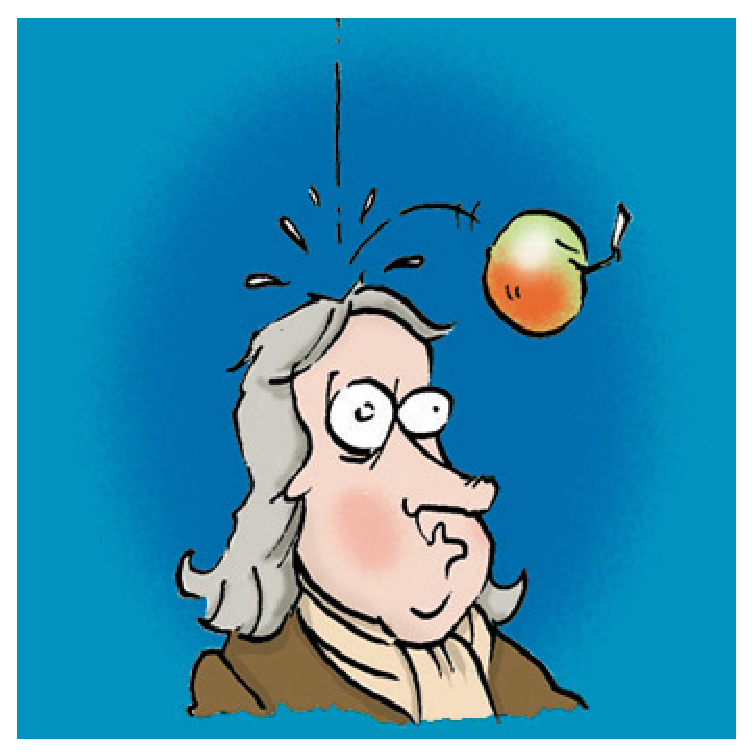
\includegraphics[height=.2\textheight]{newton}}} + 
                \vcenter{\hbox{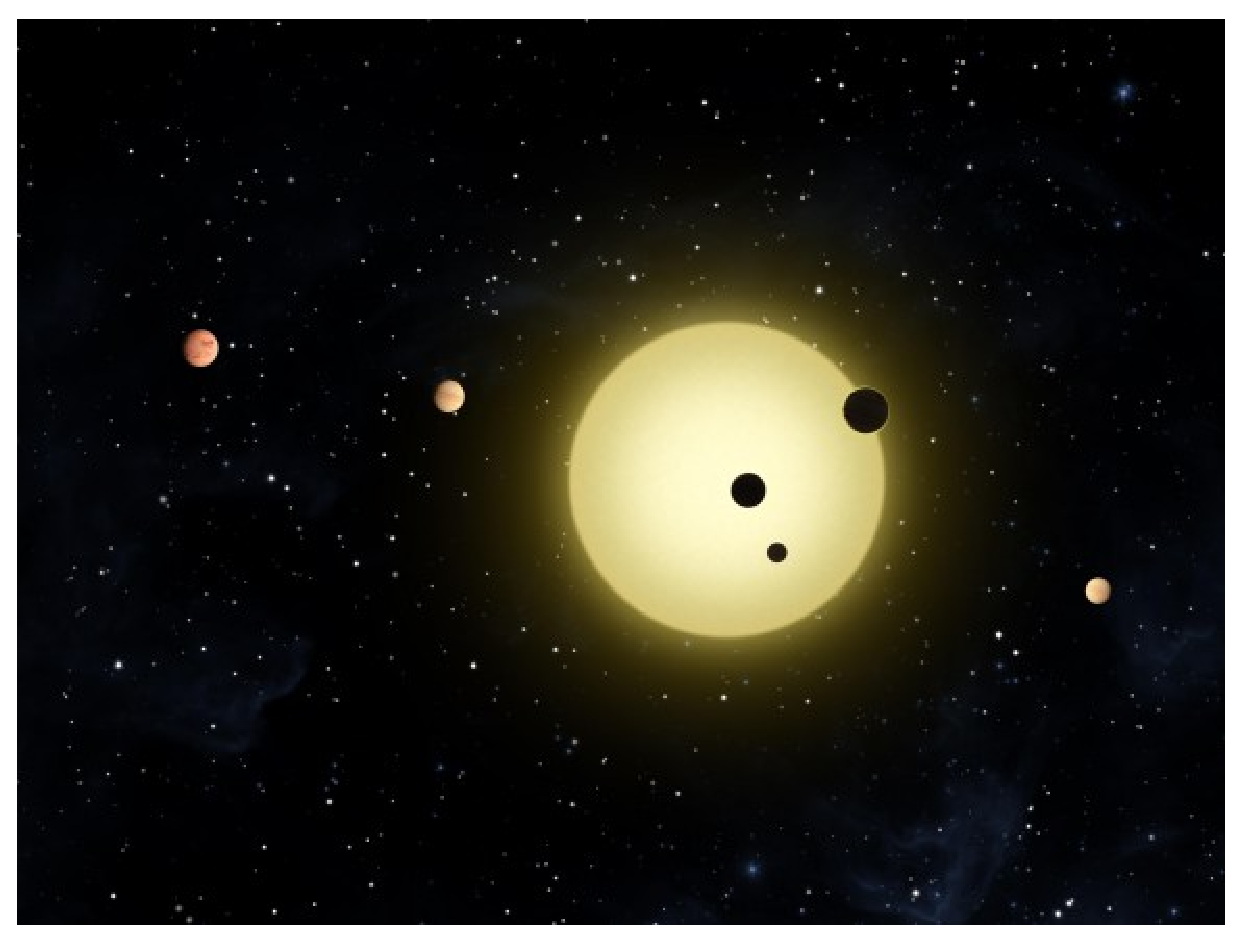
\includegraphics[height=.2\textheight]{kepler}}}$
        $\longrightarrow U(r) = -\frac{GMm}{r}$.
        \end{figure}

        Depends only on the distance $r$, simmetry under rotations.
        
        Angular momentum is constant.

        Easy equation, the orbits are ellipses.
    \end{block}
}
\end{frame}

\begin{frame}
    \frametitle{Simmetries and modern physics}
    \framesubtitle{A first success: the birth of special relativity}
    \centering
                $\vcenter{\hbox{
                    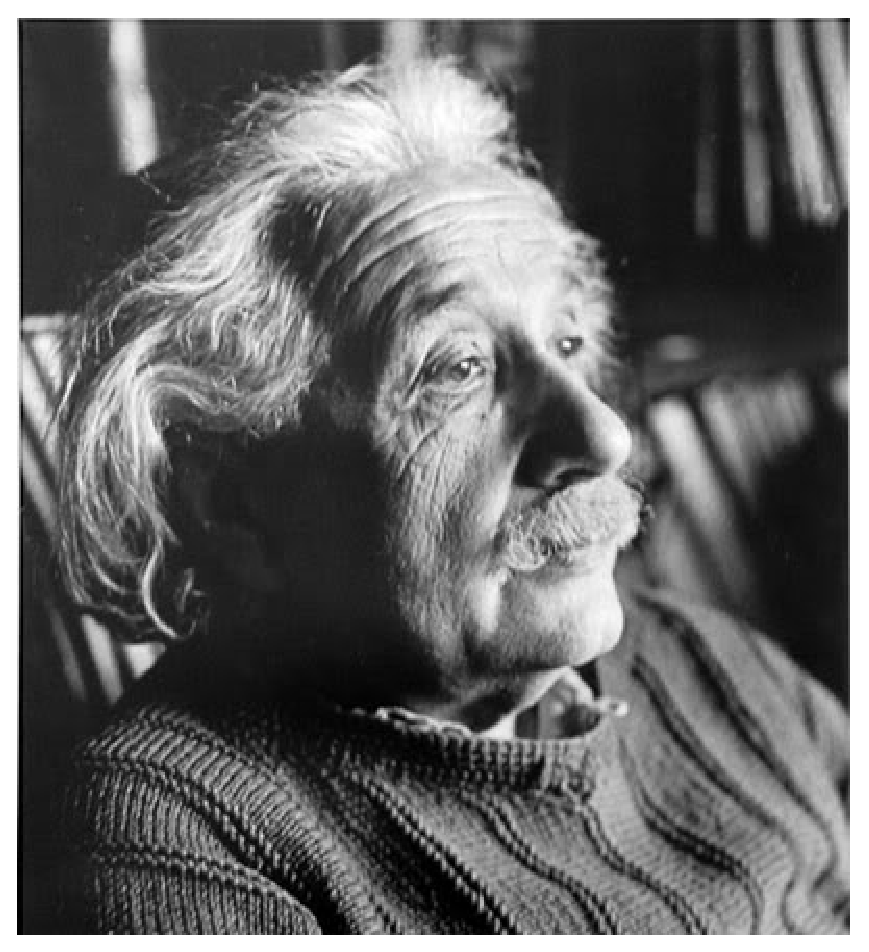
\includegraphics[height=.2\textheight]{einstein}}}$
                    \parbox{.5\textwidth}{
                    Look! Your equations have more\\simmetries than
                we expected!}
                $\vcenter{\hbox{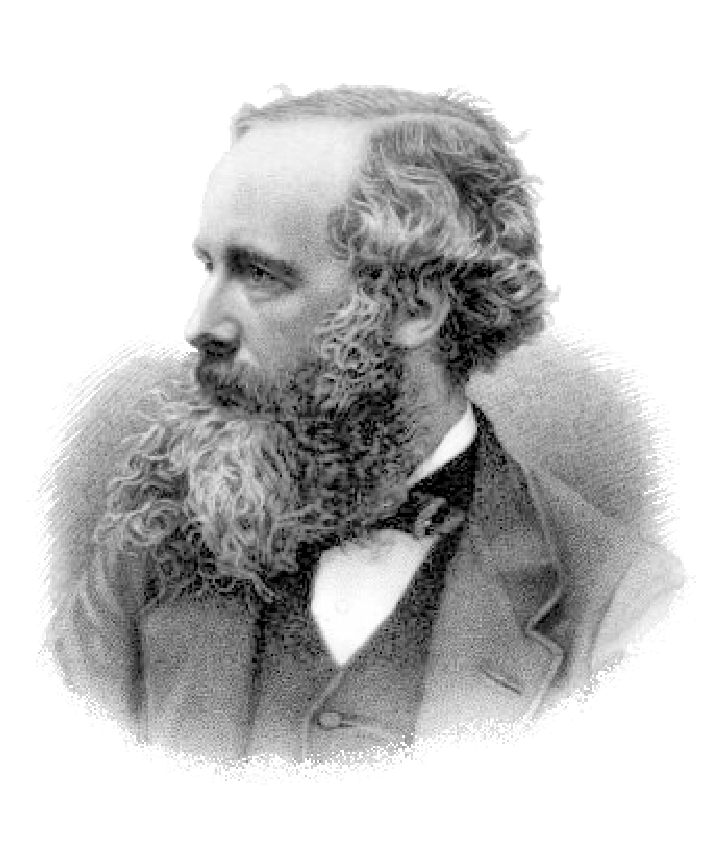
\includegraphics[height=.2\textheight]{maxwell}}}$

                \begin{align*}
                    \nabla \cdot \vec{E} &= \rho\\
                    \nabla \times \vec{B} &= \dfrac{\partial
                        \vec{E}}{\partial t} + \vec{J}\\
                        \cdots
                \end{align*}

                \uncover<2->{
                    \begin{block}{Lorentz transformations}
                        \begin{itemize}
                            \item space and time translations;
                            \item space rotations;
                            \item Lorentz boosts: $t^{'} = \dfrac{t -
                                vx/c^2}{sqrt{1 - v^2/c^2}}$.
                        \end{itemize}
                 \end{block}}
\end{frame}

\begin{frame}
    \frametitle{Simmetries first!}
    \begin{itemize}
        \item Space and time are homogeneous: no privileged points.
        \item Space is isotropic: no privileged direction.
    \end{itemize}

    What is the most general physical theory compatible with these requirements?

    \uncover<2->{Relativistic mechanics!
\begin{align*}
        E &= mc^2\\
        \frac{dp^\mu}{ds} &= eF^{\mu\nu}u_\nu\\
        \cdots
\end{align*}
}

    \uncover<3->{Unification of mechanics and electromagnetism, under the
    same simmetry principle.}
\end{frame}

\begin{frame}
    \frametitle{The Standard Model of particle physics}
    \begin{block}
        {Goal}
    Unification and full description of electromagnetic, weak nuclear force, and strong nuclear
    force.
    \end{block}
    \begin{enumerate}
        \uncover<1-> {\item symmetry principle. [$SU(3) \times SU(2) \times
            U(1)$ invariance];
        \uncover<2->{\item particles: what is the universe made of?}
    \end{enumerate}

    %\begin{figure}[h!]
            %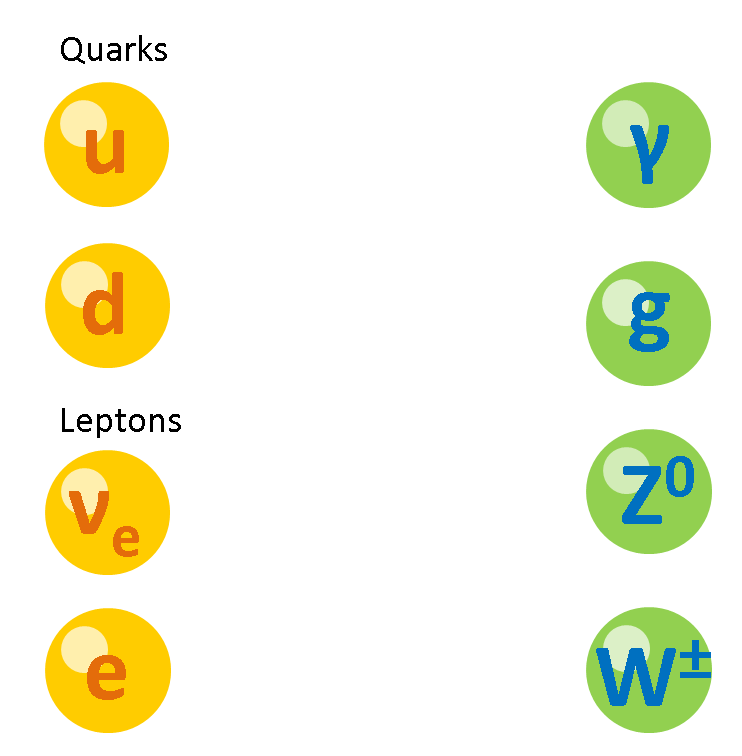
\includegraphics{standard_model_particles_1family}
    %\end{figure}
\end{frame}

\begin{frame}
    \frametitle{Why do physicists like the Standard Model}
    \begin{block}
        {Theory}
        Very few and simple premises, simmetry principles. Unbelievable
        predicting power.
    \end{block}
    \begin{block}
        {Experiment}
        Its predictions have been confirmed without exceptions to an
        astonishing degree.
        \begin{equation*}
            \dfrac{g_{\text{exp}}}{2} = 1.001 159 652 180 85(76)
            \dfrac{g_{\text{th}}}{2} = 1.001 159 652 177 60(520)
        \end{equation*}
        \begin{itemize}
            \item Incredible experimental precision: less than one part per
                trillion.
            \item Unmatched agreement between theory and experiment in the
                history of science.
        \end{itemize}
    \end{block}
\end{frame}

\begin{frame}
    \frametitle{Why do we think there is something beyond the Standard
    Model}
    \framesubtitle{The hierarchy problem}

\end{frame}<++>
\end{document}
